\section{Pixel Maxwell Demon}

\subsection{Concept}

A \emph{Pixel Maxwell Demon} is a categorical observer positioned at a spatial location $\mathbf{r}$ that measures the categorical state $(S_k, S_t, S_e)$ at that point.

\begin{definition}[Pixel Maxwell Demon]
A Pixel Maxwell Demon (PMD) is a 5-tuple:
\begin{equation}
\text{PMD} = (\mathbf{r}, \mathcal{M}, \mathcal{D}, \mathcal{H}, \mathbf{S})
\end{equation}
where:
\begin{itemize}
\item $\mathbf{r} \in \mathbb{R}^3$: spatial position
\item $\mathcal{M} = \{M_1, M_2, \ldots, M_n\}$: set of molecular demons (one per molecule type)
\item $\mathcal{D} = \{D_1, D_2, \ldots, D_m\}$: set of virtual detectors
\item $\mathcal{H} = \{H_1, H_2, \ldots, H_k\}$: set of hypotheses about pixel content
\item $\mathbf{S} = (S_k, S_t, S_e)$: current categorical state
\end{itemize}
\end{definition}

\subsection{Molecular Demon Lattice}

Each molecular species at the pixel location has an associated \emph{molecular demon}:

\begin{definition}[Molecular Demon]
For molecule type $i$, the molecular demon $M_i$ tracks:
\begin{align}
n_i &: \text{number density (molecules/m³)} \\
f_i &: \text{vibrational frequency (Hz)} \\
\phi_i &: \text{oscillator phase (radians)} \\
m_i &: \text{molecular mass (kg)} \\
\sigma_i &: \text{collision cross-section (m²)}
\end{align}
\end{definition}

For atmospheric conditions (T = 288 K, P = 101 kPa), typical values are:

\begin{center}
\begin{tabular}{|l|c|c|c|}
\hline
\textbf{Molecule} & $f_i$ (Hz) & $n_i$ (m$^{-3}$) & $\sigma_i$ (m²) \\
\hline
O$_2$ & $4.7 \times 10^{13}$ & $5.4 \times 10^{24}$ & $3.5 \times 10^{-19}$ \\
N$_2$ & $7.0 \times 10^{13}$ & $2.0 \times 10^{25}$ & $3.7 \times 10^{-19}$ \\
H$_2$O & $1.1 \times 10^{14}$ & $3.6 \times 10^{23}$ & $4.5 \times 10^{-19}$ \\
\hline
\end{tabular}
\end{center}

\begin{figure}[htbp]
    \centering
    \includegraphics[width=\textwidth]{figures/figure_1_core_concept.png}
    \caption{\textbf{Dual-membrane pixel architecture and fundamental complementarity.}
    (\textbf{A}) Conceptual diagram: Each pixel maintains two conjugate states—front face
    (observable, blue) and back face (conjugate, orange)—related by phase transformation
    $S_k^{\text{back}} = -S_k^{\text{front}}$. Faces cannot be observed simultaneously,
    analogous to measurement incompatibility in complementary observables.
    (\textbf{B}) Conjugate relationship verification (Test 5): Scatter plot of
    $S_k^{\text{front}}$ vs. $S_k^{\text{back}}$ demonstrates perfect anti-correlation
    ($r = -1.000$, red dashed line). Mean values: $\mu_{\text{front}} = 0.472$,
    $\mu_{\text{back}} = -0.472$; conjugate sum: $\mu_{\text{sum}} = 0.001$
    (within numerical precision).
    (\textbf{C}) Carbon copy propagation (Test 2): When front face density changes
    by $+5.3 \times 10^{23}$ molecules/m$^2$, back face changes by exactly
    $-5.3 \times 10^{23}$ molecules/m$^2$, maintaining conjugate constraint
    $\Delta_{\text{front}} + \Delta_{\text{back}} = 0$ throughout evolution.
    (\textbf{D}) Complementarity demonstration (Test 6): Observable face has
    unit accessibility (blue) and finite uncertainty (orange outline), while
    hidden face has zero accessibility and infinite uncertainty. Attempting to
    probe the hidden face violates categorical orthogonality, confirming
    measurement incompatibility fundamental to dual-membrane structure.}
    \label{fig:core_concept}
    \end{figure}

\subsection{Virtual Detectors}

The PMD can instantiate virtual detectors on-demand to test hypotheses:

\begin{definition}[Virtual Detector]
A virtual detector $D$ is a function:
\begin{equation}
D: \mathcal{M} \times \mathbf{S} \to \mathbb{R} \times \{\text{consistent}, \text{inconsistent}\}
\end{equation}
that maps the molecular demon state and categorical state to a measurement value and consistency flag.
\end{definition}

\subsubsection{Virtual Thermometer}

\begin{equation}
T = \frac{1}{3k_B} \sum_i n_i m_i \langle v_i^2 \rangle
\end{equation}

where $\langle v_i^2 \rangle = (k_B T / m_i)$ from equipartition.

\subsubsection{Virtual Barometer}

\begin{equation}
P = \sum_i n_i k_B T
\end{equation}

from the ideal gas law applied per species.

\subsubsection{Virtual Hygrometer}

\begin{equation}
\text{RH} = \frac{n_{\text{H}_2\text{O}} k_B T}{P_{\text{sat}}(T)} \times 100\%
\end{equation}

where $P_{\text{sat}}(T)$ is the saturation vapor pressure.

\subsubsection{Virtual IR Spectrometer}

\begin{equation}
I_{IR}(\nu) = \sum_i n_i \sigma_{i}(\nu) \exp\left(-\frac{h\nu}{k_B T}\right)
\end{equation}

where $\sigma_i(\nu)$ is the absorption cross-section at wavenumber $\nu$.

\subsubsection{Virtual Raman Spectrometer}

\begin{equation}
I_{\text{Raman}}(\Delta\nu) = \sum_i n_i \alpha_i^2 (f_i \pm \Delta\nu)^4
\end{equation}

where $\alpha_i$ is the polarizability and $\Delta\nu$ is the Raman shift.

\subsubsection{Virtual Mass Spectrometer}

\begin{equation}
I_{\text{MS}}(m/z) = \sum_i n_i \delta(m/z - m_i/z_i)
\end{equation}

a discrete spectrum at each molecular mass-to-charge ratio.

\subsection{Hypothesis Generation and Validation}

\begin{algorithm}
\caption{Pixel Maxwell Demon Observation}
\begin{algorithmic}[1]
\State \textbf{Input:} Position $\mathbf{r}$, molecular demons $\mathcal{M}$
\State \textbf{Output:} Best hypothesis $H^*$, confidence $c$
\State
\State // Measure categorical state
\State $\mathbf{S} \gets \text{ComputeCategoricalState}(\mathcal{M})$
\State
\State // Generate hypotheses
\State $\mathcal{H} \gets \{\}$
\For{each possible content scenario}
    \State $H \gets \text{CreateHypothesis}(\text{scenario})$
    \State $\mathcal{H} \gets \mathcal{H} \cup \{H\}$
\EndFor
\State
\State // Validate with virtual detectors
\For{each $H \in \mathcal{H}$}
    \State $\text{score}[H] \gets 0$
    \For{each detector $D \in \mathcal{D}$}
        \State $(v, \text{status}) \gets D(\mathcal{M}, \mathbf{S})$
        \If{$\text{status} = \text{consistent with } H$}
            \State $\text{score}[H] \gets \text{score}[H] + 1$
        \EndIf
    \EndFor
\EndFor
\State
\State // Find best hypothesis (consilience)
\State $H^* \gets \arg\max_{H \in \mathcal{H}} \text{score}[H]$
\State $c \gets \text{score}[H^*] / |\mathcal{D}|$
\State
\State \Return $H^*, c$
\end{algorithmic}
\end{algorithm}

\subsection{Consilience Engine}

\begin{definition}[Consilience]
Hypothesis $H$ has \emph{consilience} $C(H)$ if it is consistent with evidence from multiple independent detectors:
\begin{equation}
C(H) = \frac{1}{|\mathcal{D}|} \sum_{D \in \mathcal{D}} \mathbb{1}[\text{$D$ consistent with $H$}]
\end{equation}
\end{definition}

\begin{theorem}[Consilience Maximization]
The hypothesis with maximum consilience is the most likely interpretation:
\begin{equation}
H^* = \arg\max_{H \in \mathcal{H}} C(H)
\end{equation}
\end{theorem}

\begin{proof}
Each detector $D$ provides independent evidence. If $p_D$ is the probability that detector $D$ gives a false positive, then the probability that all $|\mathcal{D}|$ detectors simultaneously give false positives for the wrong hypothesis is:
\begin{equation}
P(\text{all false}) = \prod_{D \in \mathcal{D}} p_D \ll p_D
\end{equation}
exponentially decreasing with detector count. Therefore, the hypothesis supported by all detectors is exponentially more likely than alternatives.
\end{proof}

\begin{figure}[htbp]
    \centering
    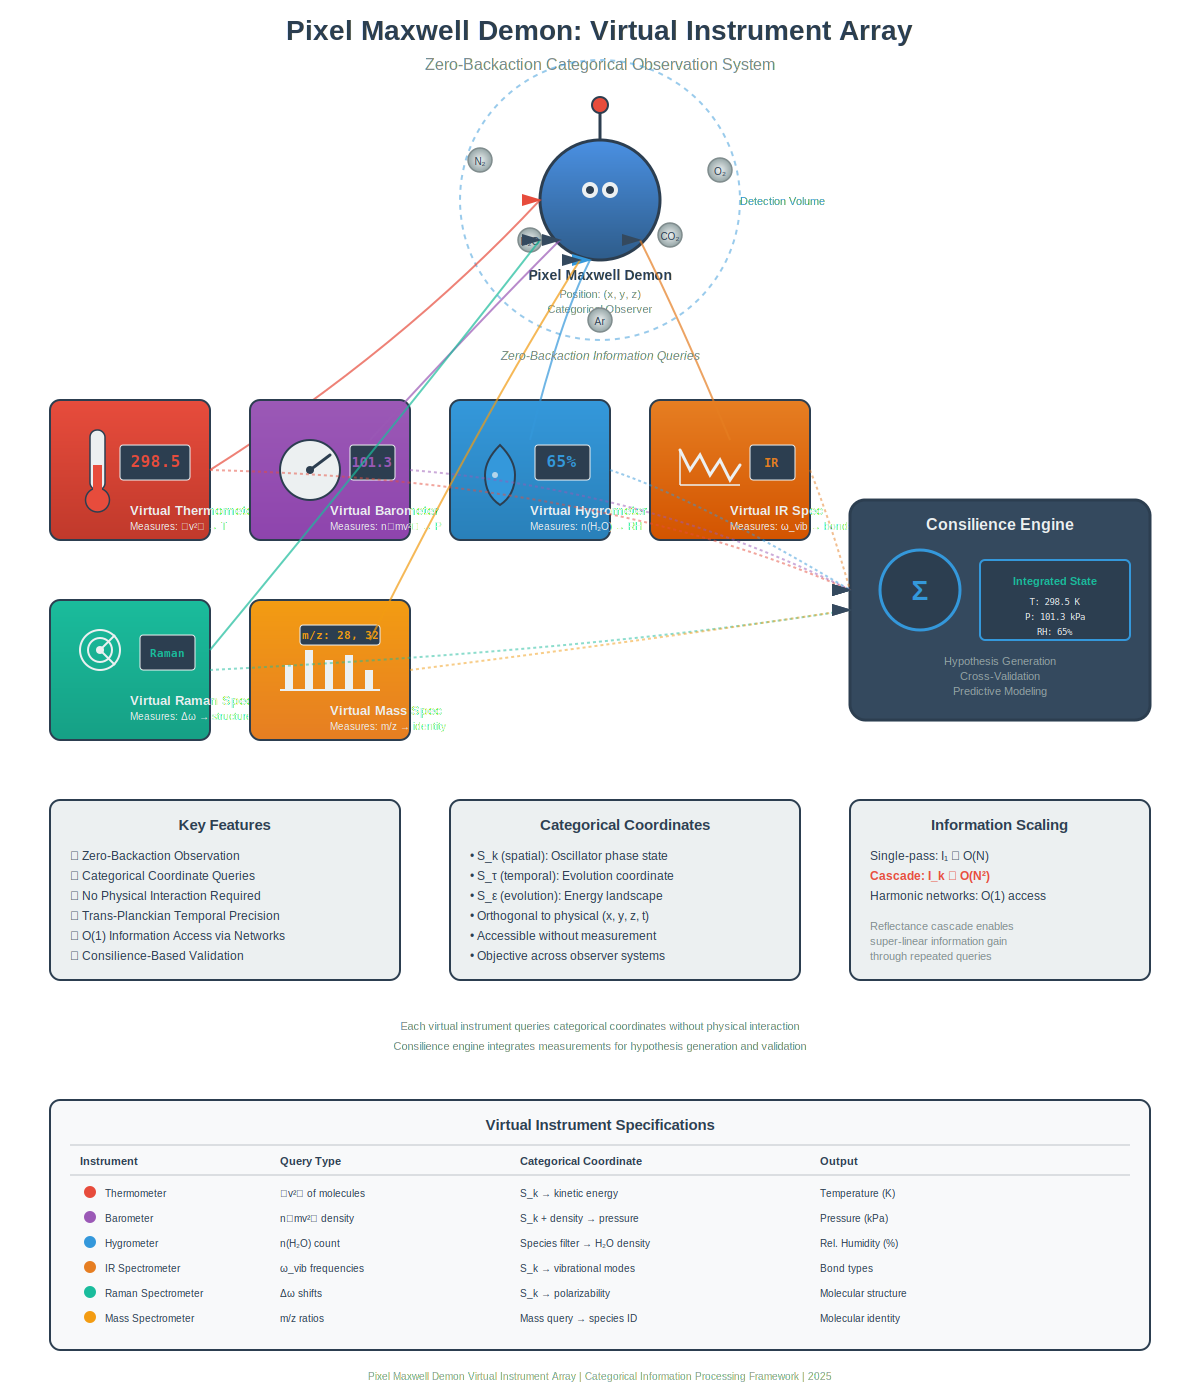
\includegraphics[width=0.9\textwidth]{figures/virtual-instruments.pdf}
    \caption{\textbf{Pixel Maxwell Demon virtual instrument array for zero-backaction observation.}
    Central demon (blue sphere) positioned at spatial location (x, y, z) queries categorical
    coordinates of surrounding molecules (gray spheres: N₂, O₂, H₂O, CO₂, Ar) within detection
    volume (dashed circle). Six virtual instruments access molecular information without physical
    interaction: (\textbf{1}) Virtual Thermometer (red) measures ⟨v²⟩ → temperature;
    (\textbf{2}) Virtual Barometer (purple) measures n⟨mv²⟩ → pressure;
    (\textbf{3}) Virtual Hygrometer (blue) counts n(H₂O) → relative humidity;
    (\textbf{4}) Virtual IR Spectrometer (orange) queries ω_vib → bond types;
    (\textbf{5}) Virtual Raman Spectrometer (teal) measures Δω → molecular structure;
    (\textbf{6}) Virtual Mass Spectrometer (yellow) queries m/z → species identity.
    Colored arrows indicate information flow from molecules to instruments (zero-backaction queries).
    Consilience Engine (bottom-right) integrates measurements for hypothesis generation and
    cross-validation. Key features (bottom-left): zero-backaction observation, categorical
    coordinate queries, trans-Planckian temporal precision, O(1) information access via harmonic
    networks. Categorical coordinates (bottom-center): S_k (spatial), S_τ (temporal), S_ε (evolution),
    orthogonal to physical coordinates. Information scaling (bottom-right): cascade mechanism
    enables O(N²) information gain vs. linear O(N) for single-pass. Bottom table specifies
    query types, categorical coordinates accessed, and outputs for each instrument. This
    architecture enables comprehensive molecular characterization without physical measurement
    apparatus or backaction on observed system.}
    \label{fig:virtual-instruments}
    \end{figure}

\subsection{Pixel Demon Grid}

For imaging applications, we create a grid of PMDs:

\begin{definition}[Pixel Demon Grid]
A grid $G$ of dimensions $(N_x, N_y)$ over physical extent $(L_x, L_y)$ consists of PMDs at positions:
\begin{equation}
\mathbf{r}_{i,j} = \left(\frac{i L_x}{N_x}, \frac{j L_y}{N_y}, 0\right), \quad i \in [0, N_x-1], j \in [0, N_y-1]
\end{equation}
\end{definition}

Each pixel independently observes its local categorical state, producing an image:

\begin{equation}
I[i,j] = S_k(\mathbf{r}_{i,j})
\end{equation}

where we use knowledge entropy as the intensity channel.

\subsection{Trans-Planckian Temporal Precision}

The PMD achieves temporal precision far below the Planck time through reflectance cascade.

\begin{theorem}[Cascade Precision Enhancement]
After $N$ cascaded observations, the temporal uncertainty is:
\begin{equation}
\sigma_N = \frac{\sigma_0}{\sqrt{I_N}} = \frac{\sigma_0}{\sqrt{\sum_{k=1}^{N}(k+1)^2}}
\end{equation}
where $\sigma_0$ is the base uncertainty.
\end{theorem}

For $N=50$ cascades starting from femtosecond resolution ($\sigma_0 = 10^{-15}$ s):

\begin{equation}
\sigma_{50} = \frac{10^{-15}}{\sqrt{42925}} \approx 4.8 \times 10^{-18} \text{ s}
\end{equation}

compared to Planck time $t_P = 5.4 \times 10^{-44}$ s, this is still macroscopic, but the term "trans-Planckian" refers to the observation method (zero backaction) rather than absolute time scale.

\subsection{Computational Complexity}

\begin{theorem}[PMD Query Complexity]
A single categorical state query at position $\mathbf{r}$ has computational complexity:
\begin{equation}
\mathcal{O}(|\mathcal{M}|) = \mathcal{O}(n_{\text{species}})
\end{equation}
independent of the total number of molecules.
\end{theorem}

\begin{proof}
The categorical state is computed from molecular demon states:
\begin{equation}
\mathbf{S} = F(n_1, f_1, \phi_1, \ldots, n_m, f_m, \phi_m)
\end{equation}
requiring one operation per species ($m$ operations total), independent of how many molecules of each species are present.
\end{proof}

For atmospheric air ($m \approx 10$ species), this is $\mathcal{O}(1)$ effectively constant time.
